% define document type (i.e., template. Here: A4 APA manuscript with 12pt font)
\documentclass[man, 12pt, a4paper]{apa7}

% add packages
\usepackage[american]{babel}
\usepackage[utf8]{inputenc}
\usepackage{csquotes}
\usepackage{hyperref}
\usepackage[style=apa, sortcites=true, sorting=nyt, backend=biber, natbib=true, uniquename=false, uniquelist=false, useprefix=true]{biblatex}
\usepackage{authblk}
\usepackage{graphicx}
\usepackage{setspace,caption}
\usepackage{subcaption}
\usepackage{enumitem}
\usepackage{lipsum}
\usepackage{soul}
\usepackage{xcolor}
\usepackage{fourier}
\usepackage{stackengine}
\usepackage{scalerel}
\usepackage{fontawesome}
\usepackage[normalem]{ulem}
\usepackage{longtable}
\usepackage{amsmath}
\usepackage{afterpage}
\usepackage{float}
\usepackage{titling}

% formatting links in the PDF file
\hypersetup{
pdfpagemode={UseOutlines},
bookmarksopen=true,
bookmarksopenlevel=0,
hypertexnames=false,
colorlinks   = true, %Colours links instead of ugly boxes
urlcolor     = blue, %Colour for external hyperlinks
linkcolor    = blue, %Colour of internal links
citecolor   = cyan, %Colour of citations
pdfstartview={FitV},
unicode,
breaklinks=true,
}

% language settings
\DeclareLanguageMapping{american}{american-apa}

% add reference library file
\addbibresource{references.bib}

% Title and header
\title{Supplemental Information B: Context of the Migration Experience Framework}
\shorttitle{SI B: Context}
\author{Jannis Kreienkamp, Kai Epstude, Laura F. Bringmann, Peter de Jonge}

% set indentation size
\setlength\parindent{1.27cm}

% adapt table and figure labels
\setcounter{equation}{0}
\setcounter{figure}{0}
\setcounter{table}{0}
\setcounter{page}{1}
\makeatletter
\renewcommand{\theequation}{S\arabic{equation}}
\renewcommand{\thefigure}{S\arabic{figure}}
\renewcommand{\thetable}{S\arabic{table}}

% Start of the main document:
\begin{document}

% add title information (incl. title page and abstract)
\begin{titlepage}
	{\noindent\Large Suppplementary Information for \par}
	\vspace{0.5cm}
	{\noindent\Large Integration of Migrants: A Descriptive Conceptual Framework and Systematic Review\par}
	\vspace{1.5cm}
	{\noindent\LARGE\bfseries \thetitle \par}
	\vspace{2cm}
	{\noindent\Large\itshape \theauthor \par}
	\vfill
	\noindent Corresponding Author Jannis Kreienkamp\par
	\noindent E-mail: j.kreienkamp@rug.nl\par
	\vfill

    % Bottom of the page
	{\noindent Last updated: \today\par}
\end{titlepage}

% add title again on page 1 (after title page)
\begin{center}
   \textbf{\thetitle} 
\end{center}

This supplementary information elaborates on the background literature of the contextual aspects of our conceptual framework presented in the main text. We would like to address each of the four contextual factors in more detail: (1) Cultures, (2) individuals, (3) situations, and (4) the process.

\begin{figure}[h]
\centering
\caption{Conceptual Model with Context. Too complex, static, and not enough focus on our key elements?}
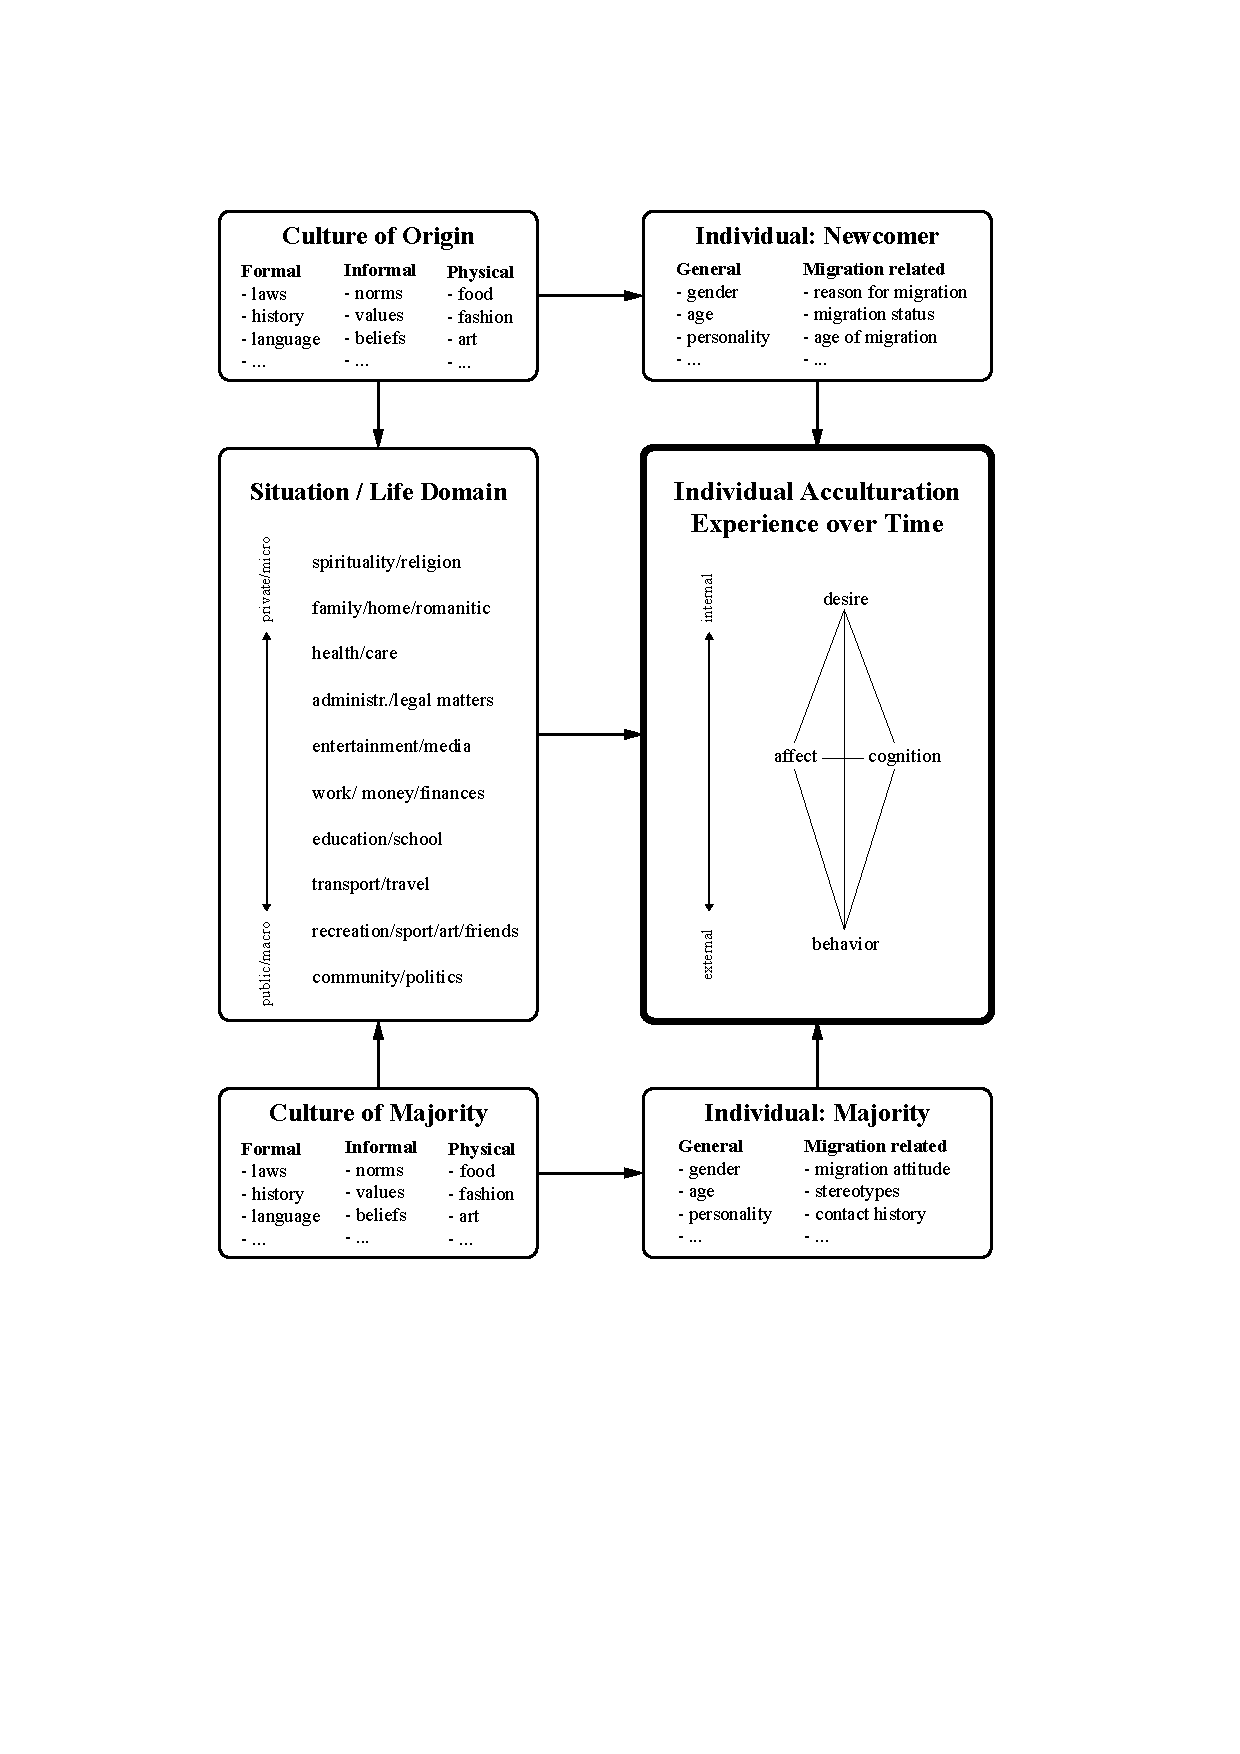
\includegraphics[width=\textwidth]{Figures/ConceptualFrameworkStatic.pdf}
\label{fig:SupModelContext}
\end{figure}

\section{Culture} 
%% Introduction Culture: 
% Culture is prominent and should be structured for a widely applicable framework.
The most prominent contextual factor of cultural adaptation is probably the role of the interacting cultures. The role of culture seems particularly important, because it becomes salient in our social lives and influences a wide variety of attitudes and behaviors, but also in social structures and institutions. 
Most (semi-)applied research projects might not need to consider or formalize the structural role of cultures -- because they can simply embed their research in the cultural context of the two particular cultures they considered.
In contrast, theories of acculturation and broader social- and cultural theories have long considered different conceptual influences of culture and society on the individual's experience. We will rely on these theories to guide our understanding of culture here. However, because our framework fundamentally relies on the individual acculturation experience, we will merely use the structuring elements of these sociological, anthropological, and psychological theories. Moreover, because these fields often use different terms to describe the same or similar concepts, our presentation here might not always be consistent with the original terminologies. Similarly, the individual theoretical and philosophical positions and implications (and their criticisms) would be beyond the scope of our paper and will thus not be discussed here.

%% Culture as social facts: 
% social facts (formal: law, regulations, policies, history, language; informal: norms, values, beliefs, [e.g., roles, moral-, religious beliefs], rituals, customs, cultural products: fashion, architecture, arts [e.g., film, music, literature, art]) relate to the affordances of ABCD
In our attempt to structure the influences of \textit{culture} we will mainly use extensions on Émile Durkheim's concept of \textit{social facts} \citep[e.g.,][]{Durkheim1982, Gilbert1989} and Berry's \textit{general framework of acculturation} \citep{Berry1997b, Berry2003, Berry2006a}. Interestingly, Durkheim's original definition of the concept of social facts directly referred to affect, behavior, and cognition (and potentially desires), when he wrote that social facts ``consist of manners of acting, thinking and feeling external to the individual, which are invested with a coercive power by virtue of which they exercise control over him'' (p. 52). Following this definition, we will mainly consider external (cultural or societal) influences that guide a person's motivational, cognitive, emotional, and behavioral experience. Within the sociological literature, these social influences can be divided into the formal social facts (e.g., laws, regulations, policies, history, language), informal social facts \citep[e.g., norms, values, beliefs, rituals, customs; also see][]{Herzog2018}, as well as more material cultural products or artifacts \citep[e.g., food, fashion, architecture, or arts, such as film, music, literature, and fine arts; e.g., see][]{Alexander2001}. The content of these external influences will likely be relevant in the expected patterns of behavior (e.g., dress or communication styles), cognition (e.g., sense of race-, class-, gender-, and sexual identities), emotions (e.g., expressions of emotions), and motivations (e.g., virtues and duties).

%% Interaction of multiple cultures: 
% Use Berry to highlight power imbalances of where once culture might be more influential than another.
In the case of cultural adaptation (at least) two sets of cultural arrangements will be influencing the experience of the individual. Quite a substantial body of literature has considered this interaction between the two cultures. For our conceptualization we will use Berry's framework for acculturation research \citep[e.g., see][p. 15, Fig. 2]{Berry1997b} and Berry's acculturation framework for stress and adaptation \citep[e.g., see][p. 45, Fig. 4.1]{Berry2006a}, because they explicitly propose to jointly consider the cultural influences on the ``acculturation experience'', which we consider here (also see Figure \ref{fig:SupModelContext}).

Once we consider this encounter of multiple cultures within the structure of culture as social facts, it also becomes apparent that there are usually considerable power imbalances between the cultures \citep[e.g., see][]{Bhatia2001}. This imbalance is especially apparent in formal or material elements, such as laws or language, but similarly extends to more informal elements, such as default expectations in communication or behavioral norms and customs. Factors such as cultural distance \citep{Triandis2001} or majority group's attitudes \citep[e.g.,][]{Berry1997b, Berry2003} might, of course, influence such power imbalances, but the structuring of both acculturation and culture encourages and facilitates reflections and discussions of these issues. As part of the analyses presented in this paper, we will offer such a reflection by extracting the cultures for which acculturation measures were validated and investigated in empirical papers. This allows us to examine how much the external influences of culture on motives, emotions, thoughts, and behaviors are reflected within structural differences of measures and definitions (that is, if we can consolidate a meaningful number of studies per cultural context).

\section{Individual} 
%% Individual based on inter-group contact and Berry: 
% Individual differences in general (e.g., age, gender) but also migration related differences (e.g., reason for migration, language proficiency)
Another contextual factor to consider during the cultural adaptation process are the interacting individuals themselves. There has been a rising focus on the idea that acculturation centers around the daily interpersonal interactions a person has with people of the other group \citep{Maxwell2017, Sam2010}. And although it can, at times, be difficult to disentangle cultural from individual influences, there are a range of personal features that likely influence the cultural adaptation process. These personal differences might relate to relatively stable individual differences, such as gender or personality, but also migration related differences, such as the reason for migration (e.g., voluntary vs. forced migration), cultural distance, or migration status. Within the migration related factor we would also include aspects that might change over the course of the adaptation process but give migrants different starting positions, such as language skills and education level.
Similar to the influences of cultures, the individual differences of the interaction partners (if there are multiple people) will likely impact the cultural adaptation. And similar to culture, individual differences likely play a role for multiple aspects of the cultural adaptation process (also see Figure \ref{fig:SupModelContext}). As part of this study, we will mainly analyze the migration relevant differences. Considering individual differences on a larger, cross-study level we will mainly extract data on the type of samples collected within the validation and the empirical papers (e.g., forced vs. voluntary, youth, or clinical samples). If we find reasonable numbers of studies with specific types of samples, we will assess whether these individual differences are related to structural differences in measures or definitions used by the authors.

\section{Situation} 
%% Situations as domains of psycho-social functioning: 
% Many theories have come up with life domains that form different cultural interaction situations.
Beyond the cultural group and the individuals, the interactions of cultural adaptation are further dependent on the situational context. One way of structuring this situational context is what we will here refer to as the \textit{domains of psycho-social functioning} -- the idea that the social experience will take place within different domains in life. There are many social-scientific theories that have discussed these spheres of life. One famous example is Bronfenbrenner's Ecological systems theory \citep{Bronfenbrenner1992}, according to which humans get into contact with others, and society at large, through a number of environmental systems that range from the closest relations (e.g., family or colleagues) to the more remote relationships (e.g., mass media or societal services). A similar framework was suggested by prominent theorists of the (structural) functionalist traditions with the concept of social institutions \citep[e.g.,][]{Turner1997}. According to these sociological theorists, it is through societal institutions (commonly: family, government, economy, media, education, healthcare, and religion) that culture is transmitted and maintained \citep[e.g.,][]{Durkheim1982}. Similar ideas for domains of interaction with society and culture have also been proposed within the acculturation literature. \citet{Arends-Toth2006, Arends-Toth2007} have, for example, suggested 15 public and private life domains (e.g., education [public], child-rearing [private]) in which acculturation takes place. Empirical research in the individual acculturation field, have also provided evidence that acculturation processes can develop separately and differently within these situational domains \citep[e.g.,][]{Arends-Toth2003a}. 

%% Point of convergence: 
% We aggregate a list of micro to macro domains from past literature.
What structurally unites the conceptualizations of life domains is the dimension of closeness to the individual. That is, most areas of life found in the literature can be arranged from the most immediate (i.e., micro or private, such as family) to the broadest levels (i.e., macro or public, including government or media). So, based on sociological theories of social institutions \citep{Durkheim1982}, literature on life domains in acculturation \citep{Arends-Toth2006, Arends-Toth2007, Zane2004}, a categorization of psychological influences by the British Psychological Society \citep{Michie2005a}, and Bronfenbrenner's Ecological systems theory \citep{Bronfenbrenner1992}, we conceptualized a range of life domains relevant to the migration process (also see Figure \ref{fig:SupModelContext}). Interestingly, most methodological and empirical authors mention explicitly which domains of acculturation they measure or very clearly focus on a limited number of domains in their measurement or definition of acculturation. As part of this study we will, therefore, extract information on the domains mentioned and measured in the literature. We will then assess whether different foci on life domains also show differences in their understanding and measurement of the motivational, emotional, cognitive, and behavioral cultural adaptation.

\section{Process} 
%% Dynamic process rather than static end-product: 
% Experience can answer this call because it can only be understood based on past experiences
A final, fundamental factor we would like to address in the cultural adaptation framework is the understanding of cultural adaptation as a dynamic process rather than a static end-product. That cultural adaptation is a developmental process, and that ``acculturation occurs when two independent cultural groups come into \textit{continuous first-hand contact over an extended period of time}'' \citep[][186]{Berry1989} seem to be a generally accepted assumption within the field. Yet, within the empirical literature, few studies have actually considered the theoretical implications of migration as a process and even fewer have methodologically followed the trajectories of migrants over time. Recent years have seen a growing awareness of this discrepancy \citep[e.g.,][]{Brown2011, Ward2019}. We believe that the experience framework of cultural adaptation, as it is presented here, is ideally suited to deal with this conceptualization as a developmental process. Philosophers of the phenomenological tradition have long highlighted that subjective experience can only be understood within the history of past experiences \citep[e.g.,][; also see Figure \ref{fig:SupModelContext}]{Heidegger1867}. In this study we apply our interest in the role of time by extracting the types of analyses (static vs. dynamic) done by the authors, and assessing whether data was collected prior to migration, after migration, or both. We will then also assess whether different traditions of data collection show differences in their understanding and measurement of the motivations, emotions, thoughts, and behaviors aspects of cultural adaptation (if the systematic review includes a reasonable number of longitudinal studies).

\printbibliography

\end{document}